\chapter{CHAI: Our candidate filtering proposal}\label{chap:chai}

\chapterQuote{\textit{``I say let the world go to hell, but I should always have my tea.''}}{--- \textit{Notes from Underground}, Fyodor Dostoyevsky}

\chapterAbstract{T}{he first step towards completing a Knowledge Graph is narrowing down an initial set of theoretically potential candidates into a smaller subset that still retains most of the promising ones. This chapter introduces CHAI, our proposal for filtering candidate triples, and it is structured as follows: Section~\ref{sec:chai-intro} introduces the chapter, Section~\ref{sec:chai-proposal} explains the criteria that CHAI uses, as well as the algorithm that it follows to create rules from them, Section~\ref{sec:chai-architecture} discusses its software architecture, Section~\ref{sec:chai-evaluation} presents our experimental validation of CHAI and the conclusions we draw from it, Section~\ref{sec:chai-limitations} delves into the practical limitations of CHAI, and Section~\ref{sec:chai-summary} concludes the chapter.}

\section{Introduction}\label{sec:chai-intro}
% In this chapter we introduce CHAI~\cite{borrego2019}, our method for generating rules that are able to filter candidate triples in the context of a KG completion process by combining a number of criteria in such a way that it optimizes a given fitness function. CHAI works by producing rules that can be applied on the initial set of candidates and produce a reduced set that contains only the promising candidate triples. Then, this set can be passed on to any fact checking technique to check the correctness of each promising candidate and identify correct triples that complete the KG. The rules produced by CHAI are based on different criteria that take the internal features of the KG into account, such as the domains and ranges of every relation in the KG, in addition to the distances between its entities.

% Additionally, we evaluate CHAI on a number of different Knowledge Graphs, and we show that it is able to achieve a good performance when dealing with all relationships in every KG under study, demonstrating that it is a generic and effective method, suitable for web-scale contexts.

% Through this chapter, we continue to follow the running example of a Knowledge Graph that was introduced in Section~\ref{sec:theo-intro}.

\section{Our proposal}\label{sec:chai-proposal}
% When completing a Knowledge Graph, there is a very large number of possible triples that are not currently in said KG and that may represent correct knowledge. In practice, this number is generally large enough to prohibit an individual evaluation of every such triple.

% For instance, let us consider a relatively small KG, with 10,000 entities and 20 possible relations. In the absence of further restrictions,\footnote{Some Knowledge Graphs, such as CS-KG~\cite{dessi2022cskg} or DBpedia~\cite{lehmann2015dbpedia}, enforce type restrictions for the entities in a triple through an ontology. While this means that many Cartesian combinations of entities and relations are no longer valid, the result is usually still in the same order of magnitude.} the theoretical maximum amount of different triples that could be present in this KG would be the Cartesian product of all possible pairs of entities and all relations, resulting in $2 \cdot 10^9$ combinations. This amount is hardly tractable through conventional means, and it only keeps scaling exponentially as the Knowledge Graph grows in size.

% To overcome this issue, we devised CHAI, a technique for candidate filtering at scale. Given a Knowledge Graph, CHAI examines it and produces a set of candidate triples big enough to include most plausible knowledge, but small enough to allow other techniques further down the KG completion workflow to handle it. We achieve this by defining a reduced set of criteria, in which each criterion is responsible for filtering out implausible triples according to a heuristic. To achieve greater expressivity and to be able to represent more complex restrictions, CHAI progressively combines these criteria into rules of a fixed format, and assesses the quality of the rule after every step. These rules are produced on a per-relation basis, and thus CHAI is able to adapt them to the particularities of every relation in a Knowledge Graph.

% In the following subsections, we describe these elements in detail, as well as the algorithm that is used to produce such rules.

\subsection{Proposed criteria and rules}
% We propose a set of criteria for filtering candidates for a given Knowledge Graph $\KGlong$, where every criterion defines a heuristic to quickly reject a triple if it is considered implausible, doing so with a reduced computational cost. 

% Each criterion, thus, assigns a binary label to a candidate triple, denoting whether the candidate is rejected or accepted. A negative label means that, according to the criterion, the triple should be discarded immediately, while a positive label indicates that the triple may be interesting and should be allowed to continue further down the KG completion workflow. Each criterion is devised following a different approach, and therefore the sets of candidates that are allowed by each of them are relatively disjoint, although they might overlap to some extent. 
% We further discuss the derived implications of this fact in Section \ref{sec:chai-limitations}. 

% These criteria, and their associated rationales, are as follow:

% \candfunc{Criterion 1. Existing source entity and relation}{
%     Let $(s,r,t)$ be a candidate triple. This criterion accepts the candidate if there exists a triple in \Tset{} with the same source entity and relation as the candidate. We denote this criterion as:
%     \begin{equation*}
%         \centering
%         \label{crit:exists}
%         exists_\KG((s,r,t)) \Leftrightarrow \exists~e \in \Eset \mid (s,r,e) \in \Tset
%     \end{equation*}
% }

% This criterion was devised as a response to the observation that many Knowledge Graphs do not have an ontology that restricts which entity types are allowed to be combined through a given relation. As a consequence, it is highly likely that a random combination of a source entity and a relation will be nonsensical: in the running example shown in Figure~\ref{fig:kg-potter}, a random combination of source entity and relation may result in a real-life person having a movie prequel, or a book writing another book. It follows that allowing only candidate triples whose source and relation have already been observed before in correct triples will immediately discard many of such nonsensical instances.

% \candfunc{Criterion 2. Target is in the domain of a relation $rel \in \Rset$}{
%     Let $(s,r,t)$ be a candidate triple. This criterion accepts the candidate if its target entity appears at least once as the source of an existing triple that has $rel$ as its relation. We denote this criterion as:
%     \begin{equation*}
%         \centering
%         \label{crit:dom}       
%         dom_{\KG, rel}((s,r,t)) \Leftrightarrow \exists~e \in \Eset \mid (t,rel,e) \in \Tset
%     \end{equation*}
% }

% Contrary to the previous criterion, which operates solely on a candidate triple, this one also requires a relation to be specified. Given that most impossible combinations of source and relation will be rejected by the former criterion, this one focuses on restricting which entities are allowed to appear on the right side of a candidate triple. Generally, acceptable target entities will have a certain type or belong to a union of types. However, type information is not always readily available. 

% This criterion aims to provide a similar constraint even if the KG lacks type information, by only accepting candidates whose target entities appear as a source for a given relation somewhere in the KG. This allows CHAI to leverage the implicit type restrictions that will be in place by the already existing, correct knowledge: for example, it may deduce that entities that appear as the source of the relation \textit{plays} are actors, even if this knowledge is not explicitly laid out.

% \candfunc{Criterion 3. Target is in the range of a relation $rel \in \Rset$}{
%     Let $(s,r,t)$ be a candidate triple. This criterion accepts the candidate if its target entity appears at least once as the target of an existing triple that has $rel$ as its relation. We denote this criterion as:
%     \begin{equation*}
%         \centering
%         \label{crit:ran}  
%         ran_{\KG, rel}((s,r,t)) \Leftrightarrow \exists~e \in \Eset \mid (e,rel,t) \in \Tset
%     \end{equation*}
% }

% This criterion complements the previous one by only accepting candidates whose target entity is in the range of an existing relation in the KG. Again, this leverages implicit type information present in the KG to further remove non-plausible candidates. 

% Following the example introduced in Figure~\ref{fig:kg-potter}, thanks to this criterion, one could establish that any candidate triple for the relation \textit{starred\_in} should have a target entity that is also a target of the relation \textit{has\_prequel}, due to the fact that the range of both relations is generally comprised of movies. Thus, one can immediately discard the potential candidate \tripleSty{(Emma Watson, starred\_in, Daniel Radcliffe)} because the entity \textit{Daniel Radcliffe} never appears as a target for the relation \textit{has\_prequel}.

% \candfunc{Entities are within distance $i$}{
%     Let $(s,r,t)$ be a triple in $\Tset$. This criterion selects all candidates whose source and target entities have a distance between them that is at most $i$:
%     \begin{equation*}
%         \centering
%         \label{crit:dist}  
%         dist_{\KG, i}((s,r,t)) \Leftrightarrow dist(\KG, s, t) \le i
%     \end{equation*}
% }

% Finally, this criterion covers the assumption that a good candidate triple should be such that its source and target entities are close each other in the Knowledge Graph, which has been repeatedly shown correct by related literature~\cite{borrego2021, ferre2019, oh2018, bansal2019a2n, bansal2020negatives, kong2019}.

% While the previously introduced criteria could be useful on their own, it seems reasonable that a more complex combination of them could achieve both a higher expressivity and a more satisfactory candidate filtering performance. To achieve this, CHAI combines them into candidate filtering rules of the following format, where $c_i$ are criteria other than $exists_\KG$:

% \begin{equation*}
%     \centering
%     exists_\KG~\wedge (c_1 \vee c_2 \vee \ldots \vee c_n)
% \end{equation*}

% By enforcing the $exists_\KG$ criterion on all candidate triples, we can make sure that the resulting set of candidates has a lower number of incorrect or noisy candidates, as all of them have a combination of source entity and relation that already exists in the original KG while still allowing all possible target entities. In addition, the disjunction of criteria present in the rule allows for more flexibility: longer rules with more criteria are less strict, and thus produce more candidates by combining different criteria. The following subsection illustrates the process of creating such rules.

\subsection{Algorithm}\label{sec:chai-algorithm}
% The algorithm that we propose for generating rules for candidate filtering is shown in Algorithm \ref{algo:chai}, and further described in the following. It receives the set of candidates to be filtered, the original KG in the form of a training and a testing split and a relation as input, and it outputs the generated rule for the relation.

% \begin{algorithm}[!htp]
    \DontPrintSemicolon
    \SetKwBlock{Begin}{function}{end function}
    \KwIn{
      $\KG_{trn} = (\Eset, \Rset, \Tset_{trn})$ : Training split of the KG\newline
      $\KG_{tst} = (\Eset, \Rset, \Tset_{tst})$ : Testing split of the KG\newline
      $candidates$ : Set of potential candidates to be filtered\newline
      $rel$ : Selected relation in $\Rset$\newline
      ${\ff}itness$ : Fitness function\newline
      $N$ : Maximum distance value for distance-based criteria\newline
      $\theta$ : Fitness threshold value
    }
    %\BlankLine
    \KwOut{
      $rule$ : Generated rule
    }
    \BlankLine
    \Begin($\text{CHAI} {(} \KG_{trn}, \KG_{tst}, candidates, rel, {\ff}itness, N, \theta {)}$){
      // Select the candidates in which the relation $rel$ appears\;
      $rc \gets \{(s, r, t) \in candidates \mid r = rel \}$\;
      // Initialize the rule to initially contain only $exists_{\KG_{trn}}$\;
      $rule \gets exists_{\KG_{trn}}$ \;
      // Obtain a set of initially filtered candidates by applying\;
      // $exists_{\KG_{trn}}$\;
      ${\ff}c \gets$ apply $exists_{\KG_{trn}}$ to $rc$\;\label{algo:initial-filter}
      
      \BlankLine
      
      // Add all possible criteria to the set of available criteria\;
      // using the training split of the KG\;
      $criteria \gets \emptyset$\;
      \ForAll{$r \in \Rset$, $i \in [1..N]$}{
        $criteria\gets criteria \cup \{dom_{\KG_{trn}, r}, ran_{\KG_{trn}, r}, dist_{\KG_{trn}, i}\}$ \;
      }
      
      %\BlankLine
      // Sort all criteria by the fitness value obtained on the set of\; 
      // filtered candidates they generate, using the testing split\;
      $criteria \gets$ sort $criteria$ by ${\ff}itness(\KG_{tst}, {\ff}c,$ apply $criteria$ to ${\ff}c)$ \;
  
      \BlankLine
      \ForAll{$criterion \in criteria$}{\label{algo:for-main}
          // Apply the rule to obtain a set of filtered candidates\;
          $selected\_candidates \gets$ apply $rule$ to ${\ff}c$ \;
          // Compute the fitness value of the previous set\;
          // using the testing split\;
          \If{${\ff}itness(\KG_{tst}, {\ff}c, selected\_candidates) < \theta$}{
              // Add current criterion if the threshold is not met\;
              $rule \gets $ add $criterion$ to $rule$\;
          }
      }
      
      \Return{$rule$}
    }
    \caption{CHAI} \label{algo:chai}
  \end{algorithm}
  
  

% First, the input set of candidates is narrowed down to only those that include the relation for which CHAI is being applied. This serves a dual purpose. On the one hand, since rules are produced and applied on a per-relation basis, this immediately discards any candidates that contain a different relation, which would not have been allowed anyway. On the other hand, this allows CHAI to only take into account the triples in which the desired relation is present, resulting in a more specialized rule.

% Subsequently, a rule that contains only the $exists_{\KG}$ criterion is generated, and the set of candidates that results from applying it is obtained, which will be further refined by adding more criteria to the rule. By definition of $exists_{\KG}$, this will result in a set of triples whose combination of source and relation are already present somewhere in the KG, and all possible entities as targets.

% Then, a set of criteria is instantiated, which contains the $dom$ and $ran$ criteria for every possible relation in the KG, as well as the $distance$ criterion for up to a certain maximum distance. These criteria are the ones that will be used for building the rule, however, not every criterion in the set has necessarily to be added to the rule.

% Following the previous step, a fitness value is computed for each criterion, by applying a certain fitness function on the set of candidates that are selected by that criterion. The previous set of criteria is then sorted in descending order of the fitness value that is obtained in this manner.

% Finally, these ordered criteria are added in an iterative fashion to the rule under generation, starting with the one that obtains the highest fitness value. Every time a criterion is added to the rule, the resulting set of filtered candidates produced by it is computed, and the fitness value associated with the rule is updated. This process is repeated until the fitness value exceeds a given threshold or the set of available criteria is depleted, at which point no more criteria will be added to the rule. Once this process ends, the generated rule is returned.

% In Table \ref{table:chai-iterations}, we present an example on the process of generating a rule for the relation \textit{plays}, with a threshold $\theta = 0.95$. Through the process, different criteria are iteratively added to the rule, and the fitness value is included for every step. Once the fitness value meets or exceeds the threshold, the process ends and the rule is returned. In this case, selecting candidate triples whose target entities represent people would provide a good result.

% \begin{table}
    \begin{center}
    \begin{tabular}{ M{4cm} | M{1.9cm} | M{2.5cm} } 
    \centering \textbf{Rule} & \textbf{Fitness value} & \textbf{Meets threshold?} \\
    \hline
    $exists_{\KG}~\wedge$ & - & - \\ \hline 
    $(\,ran_{\KG, created}~\vee$ & 0.80 & No \\ \hline 
    $dom_{\KG, appears\_in}~\vee$ & 0.92 & No \\ \hline 
    $dist_{\KG, 2}\,)$ & 0.96 & Yes \\ \hline 
    \end{tabular}
    \caption{An example rule being built for the relation \textit{plays}}\label{table:chai-iterations}
    \end{center}
\end{table}

% Since an integral KG completion process involves every relation in the KG, CHAI should be applied once for each relation in the KG, in order to produce the complete set of rules and suitable candidates for KG Completion. This results in a total set whose size is significantly smaller than that of the input set of candidates, while still containing as many suitable candidates as possible.

\section{Software Architecture}\label{sec:chai-architecture}

% The classes that comprise the architecture of CHAI are shown in Figure~\ref{fig:chai-diagram}, while its workflow is described in Figure~\ref{fig:chai-flow}. In the following, we further describe the architecture of CHAI: 

% \begin{figure}[htp]
%     \centering
%     \includesvg[width=1.0\textwidth]{fig/chai/CHAI-classes}
%     \caption{Architecture of CHAI}
%     \label{fig:chai-diagram}
% \end{figure}

% \begin{figure}[htp]
%     \centering
%     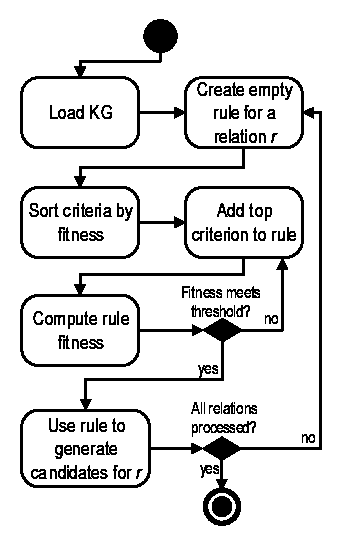
\includegraphics[width=.35\textwidth]{fig/chai/CHAI-flow}
%     \caption{Workflow of CHAI}
%     \label{fig:chai-flow}
% \end{figure}

% Class \textit{CriteriaCatalogue} contains all the available criteria that can be used to build candidate filtering rules, which can be obtained using the method \textit{getAll}. Criteria are implemented using the class \textit{Criterion}. The method \textit{apply} of this class receives a set of candidate triples, and produces a smaller, filtered set of candidates that meet the criterion in question. For example, a criterion may determine that a triple is a valid candidate if its source and target entities are less than three hops apart in the KG.

% Class \textit{FitnessFunction} is used to implement a given fitness function, which gives a numerical score to a given set of candidate triples using the \textit{evaluate} method. Some possible examples of fitness functions are the relative number of total candidate triples against the number of triples in the KG, or the percentage of candidate triples that are present in the validation split of a KG and thus more likely to be correct.

% The \textit{RuleGenerator} class is responsible for generating a candidate filtering rule for a given relation. A rule, as described in Section \ref{sec:chai-proposal}, is a conjunction of criteria that determine whether a given triple is a valid candidate or not. 

% First, a new rule is produced using the \textit{getNew} method. Then, a series of criteria are iteratively added to it in order to progressively construct it. This is done by sorting all the available criteria according to the fitness function, and then using the \textit{addCriterion} method to add the top criterion. The fitness of the resulting rule is subsequently evaluated using the \textit{evalRule} method, and this process is repeated until \textit{evalRule} returns a fitness value that meets a certain threshold.

% Finally, the \textit{Rule} instance produced by the \textit{RuleGenerator} can be used to filter candidate triples in a KG, using its \textit{apply} method. The \textit{CandidateGenerator} class handles this process, applying a given rule to the desired set of candidates and returning the set of triples that are considered promising candidates according to the rule.

\subsection{Design and performance considerations}
% The software architecture of CHAI has been devised using a number of common software patterns. First, given that only one instance of most classes is needed at runtime, all such classes have been designed as singletons, to statically guarantee a smaller memory footprint. 
% However, there are two places where a singleton cannot be used. One of them is for class Rule, since the execution of CHAI will result in the generation of one rule per relation in the KG. Another similar case is class Criterion, because it is clear that multiple different criteria should be instantiated at runtime.

% To facilitate the inclusion of new criteria in the future, they are accessed through a CriteriaCatalogue class, which takes care of detecting all available criteria in the system and loading them at runtime. This way, no further changes in the system are needed if additional criteria need to be added.

% Finally, the way in which candidates are obtained from a rule enjoys a significant optimization. Rather than following a filtering approach, where the entire set of possible candidates needs to be instantiated and then pruned, we follow a generative approach. The CandidateGenerator class is able to inspect the conditions of a rule, and then generate exclusively those candidate triples that would have been allowed by it. While the final set of filtered candidates can be proved to be the same, this results in significant runtime and memory usage improvements.

\section{Evaluation}\label{sec:chai-evaluation}
% In this section we present the experimental results that confirm that CHAI is effective in practice. First, we introduce the experimental setting. Then, we present the results of applying CHAI on several well-known Knowledge Graphs, comparing them against those of a state-of-the-art baseline technique by \citet{shi18}, which is, to the best of our knowledge, the only KG completion proposal that includes a well-defined way to filter candidate triples and experimental results on this regard. Finally, we discuss these results.

\subsection{Setup and experimental data}

% We evaluated CHAI using a number of different Knowledge Graphs that are openly available and commonly used for the task of KG completion: FB13, WN11 \cite{socher2013}, WN18 \cite{bordes2014} (which are subsets of Freebase \cite{bollacker2008} and Wordnet \cite{miller1995}, respectively), a subset of NELL introduced by \citet{gardner2015}, and EPSRC\footnote{\url{http://epsrc.rkbexplorer.com}}, which contains information about the grants provided by the Engineering and Physical Sciences Research Council of the United Kingdom. All of these Knowledge Graphs were obtained from the publicly available AYNEC-DataGen tool \cite{ayala2019}, and an overview of their metadata can be found in Table~\ref{table:chai-datasets}. We used CHAI to generate rules for every relation in every KG, except for the case of NELL, in which we focused on the same subset of 10 relations as \citet{gardner2015} due to the high number of total relations. All experiments were conducted on a computer with 32GB of RAM and an Intel Core i9-9900K CPU.

% \begin{table}[htp]
    \begin{center}
    \begin{tabular}{ M{2.5cm} | M{2.5cm} | M{2.5cm} | M{2cm} } 
    \centering \textbf{KG} & \textbf{Training triples} & \textbf{Test triples} & \textbf{Relations} \\
    \hline
    FB13 & 285,208 & 78,490 & 13 \\ 
    \hline 
    WN18 & 117,160 & 58,564 & 18 \\
    \hline 
    NELL & 201,870 & 13,491 & 519 (10) \\
    \hline 
    EPSRC & 341,372 & 85,337 & 20 \\
    \end{tabular}
    \caption{Overview of the KGs used for evaluating CHAI}
    \label{table:chai-datasets}
    \end{center}
\end{table}

% The results of the approach followed by \citet{shi18} were used as a baseline. Their proposal consists in generating candidate triples by altering the target entities of the triples already present in the KG, and replacing them by all entities that can be found in the range of the relation present in the triple. This is equivalent to applying only the $ran_{\KG, r}$ criterion, where $r$ is the relation for which CHAI is being applied. %Therefore, we obtained the baseline results by modifying CHAI to include only that criterion.

\subsection{Evaluation parameters}\label{sec:impl-details}
% To conduct our experiments, we set the distance threshold $N$ for the $distance$ criterion to 4. This value was chosen empirically, aiming to allow for a threshold as high as possible while still being reasonable in terms of computation time. Additionally, these distances were computed on a partially undirected version of the KGs. This was done to fully exploit the highly relational nature of KGs, while still not allowing paths that would be connected by means of entities with a very high in-degree such as genders or nationalities.

% The training and testing splits of the KGs were already provided by the KGs that we used, and thus we provided CHAI with these splits as is. We evaluated CHAI using a fitness function that combines reduction rate (rr) and coverage using their harmonic mean, as shown in Eq. \ref{eq:fitness-recall-rr}. The $\theta$ threshold value required by the algorithm was set to 0.99, so as to allow CHAI to find highly satisfactory rules, and to study the evolution of the coverage and reduction rate of said rules if they keep growing in size without meeting the threshold. Formally, they are defined as follows:

% \begin{equation*}
% \centering
% \begin{aligned}
% \textrm{Let}~\Sset~\textrm{be a candidates set, and}~\Sset'\subseteq \Sset~\textrm{a set of filtered candidates:}
% \end{aligned}
% \end{equation*}

% \begin{equation}
% \label{eq:fitness-recall-rr}
% \begin{gathered}
% {\ff}itness(\KG, \Sset, \Sset') = \frac{2 \cdot rr(\Sset, \Sset') \cdot coverage(\KG, \Sset')}{rr(\Sset, \Sset') + coverage(\KG, \Sset')}\textrm{\,,~where}
% \end{gathered}
% \end{equation}

% \begin{equation*}
% \label{eq:rr}
% \begin{gathered}
% rr(\Sset, \Sset') = 1 - \frac{|\Sset'|}{|\Sset|}
% \end{gathered}
% \end{equation*}

% \begin{equation*}
% \label{eq:recall}
% \begin{gathered}
% coverage(\KG = \KGlong, \Sset') = \frac{|\Sset' \cap \Tset|}{|\Tset|}
% \end{gathered}
% \end{equation*}

% This fitness function was devised under the following rationale: focusing only on coverage would result in very long rules that allow as many candidates as possible, however, this would not be desirable as we aim to reduce the size of the set of candidates, to avoid having to evaluate low-quality candidates. Conversely, focusing only on reduction rate would yield very short (and thus more restrictive) rules. As a consequence, this fitness function achieves a compromise between reduction rate and coverage, and allows for more flexibility in the lengths of the rules in contrast to focusing only on one objective. To illustrate this difference, we have also tested CHAI using two alternative fitness functions: only coverage, and only reduction rate. The results achieved by every fitness function are shown in Figure \ref{fig:chai-points-datasets}.

\subsection{Results and discussion}
% In the following, we present the results achieved by CHAI on the KGs under evaluation and the conclusions we draw from them.

% Figure \ref{fig:chai-fitness-datasets} reports on the evolution of the coverage and reduction rate for all KGs under study as rules grow in size, where each line represents a different relation; while Figure \ref{fig:chai-points-datasets} display the values for the coverage and reduction rate for every iteration in all Knowledge Graphs as points in a 2-dimensional space. Finally, Table \ref{table:recall-rr-max} provides an overview on the average maximum coverage and reduction rate that CHAI achieves for the relations in all KGs under study. This Table also includes the average coverage and reduction rate values achieved by the proposal of Shi and Weninger~\cite{shi18}, which was denoted as ``baseline'' for brevity.

% \begin{figure*}[htp]
%     \centering
%     \def\subfigscale{0.4}
%     \subfigure[FB13 - Coverage]{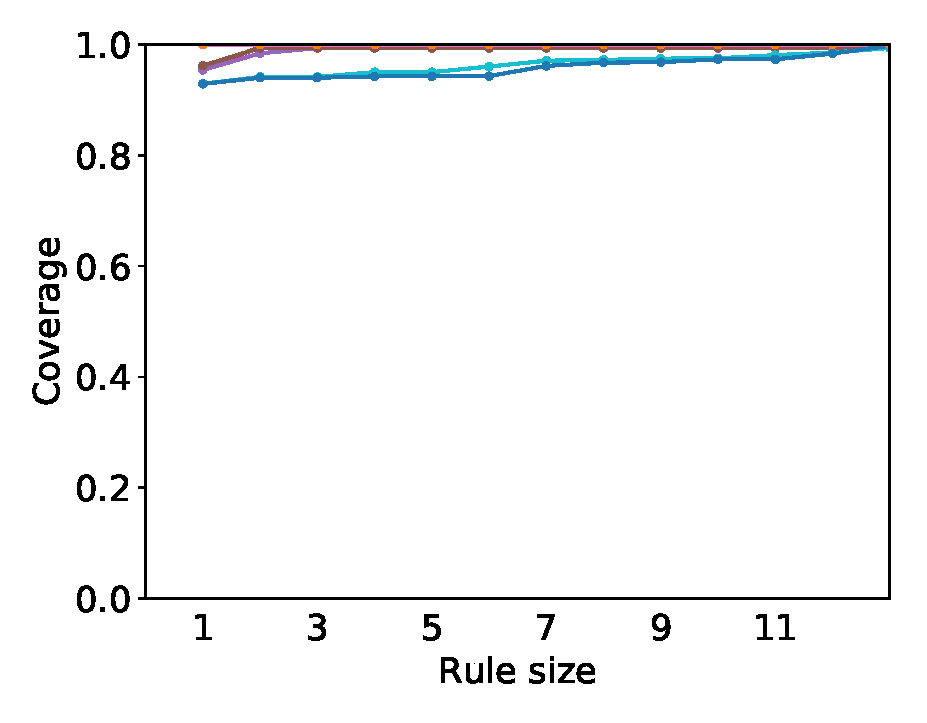
\includegraphics[scale=\subfigscale]{fig/chai/FB13_recall}\label{fig:res-FB13-recall}}~
%     \subfigure[FB13 - Reduction rate]{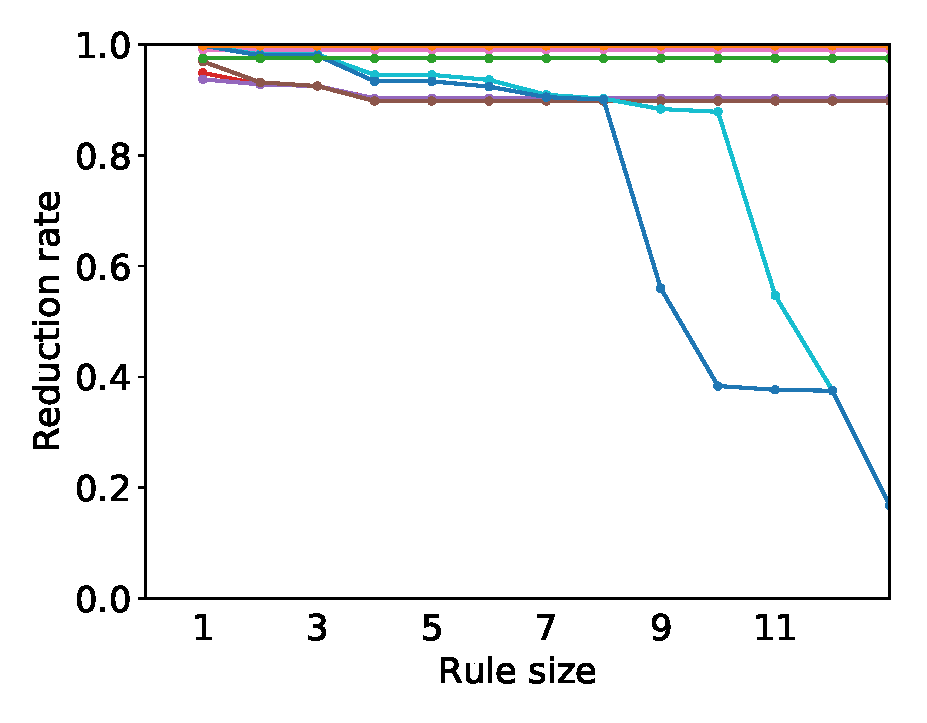
\includegraphics[scale=\subfigscale]{fig/chai/FB13_rr}\label{fig:res-FB13-rr}}\\

%     \subfigure[WN18 - Coverage]{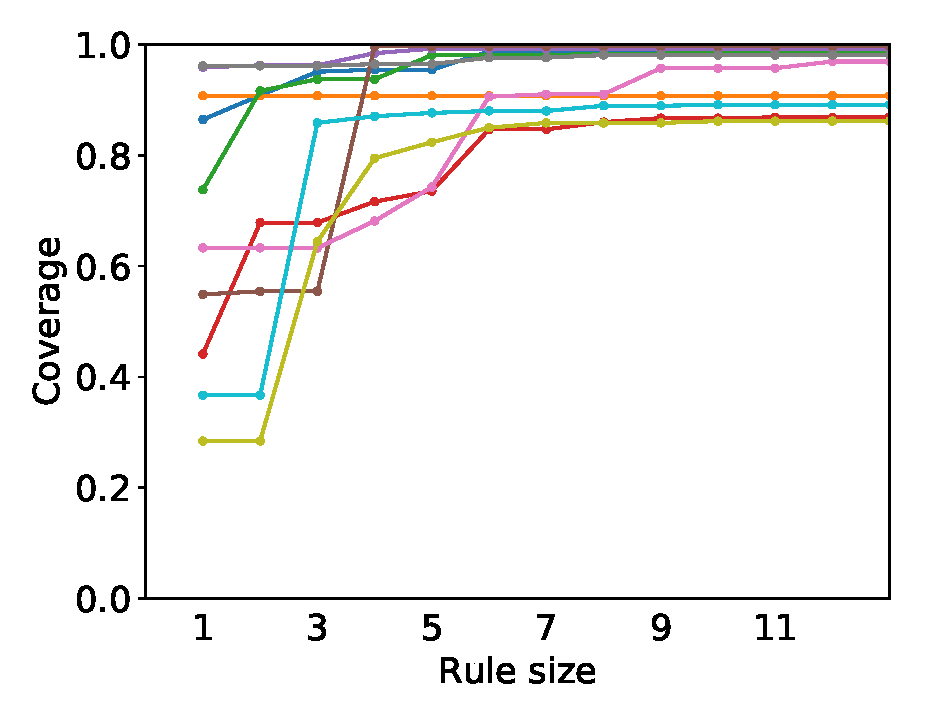
\includegraphics[scale=\subfigscale]{fig/chai/WN18-AR_recall}\label{fig:res-WN18-recall}}~
%     \subfigure[WN18 - Reduction rate]{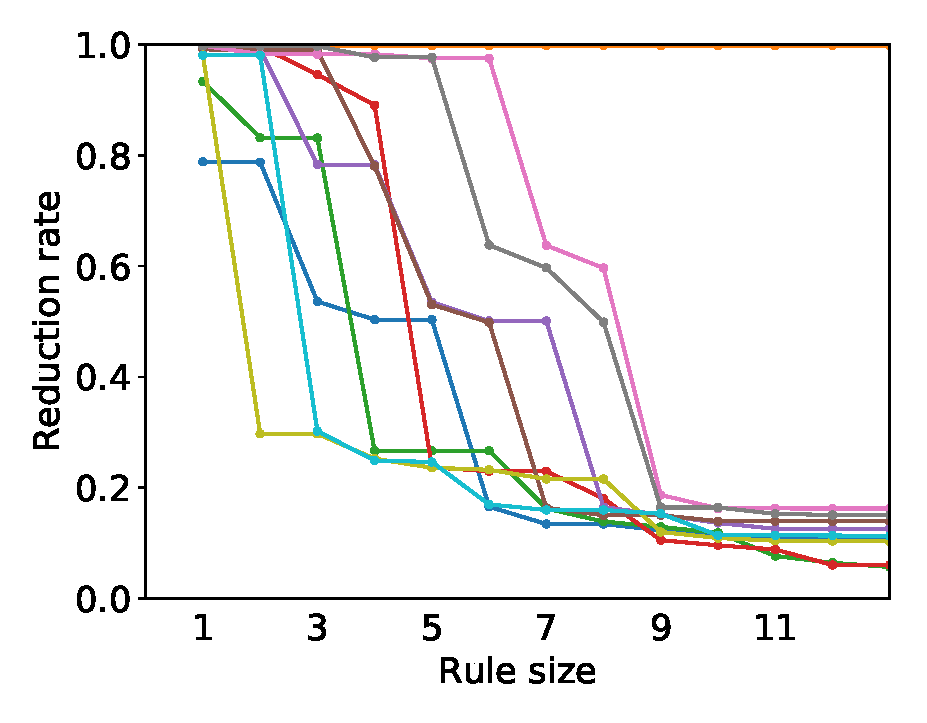
\includegraphics[scale=\subfigscale]{fig/chai/WN18-AR_rr}\label{fig:res-WN18-rr}}\\

%     \subfigure[NELL - Coverage]{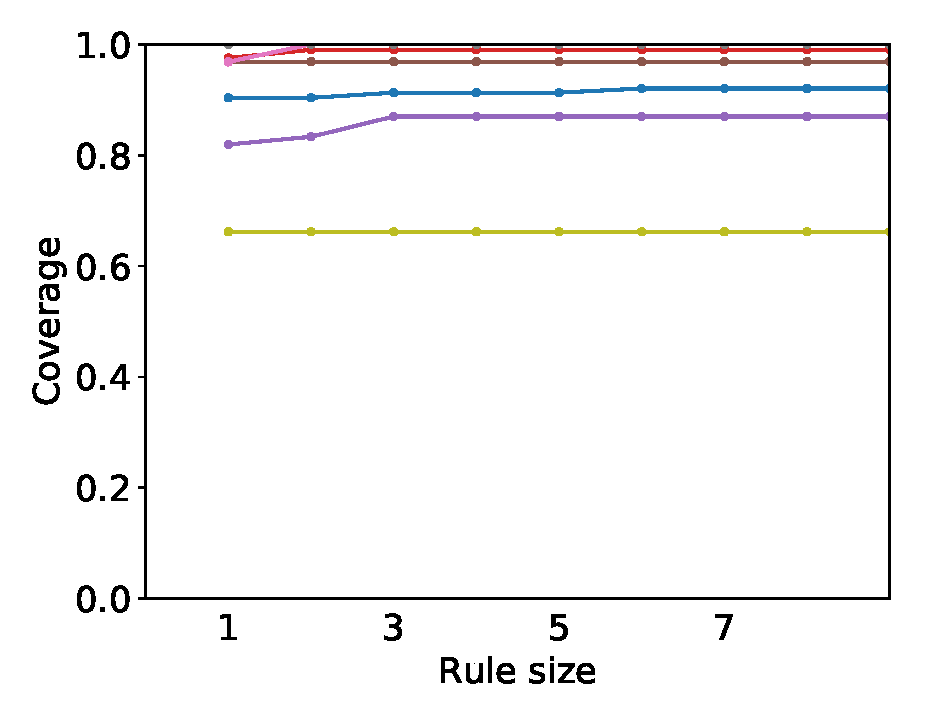
\includegraphics[scale=\subfigscale]{fig/chai/NELL-AR_recall}\label{fig:res-NELL-recall}}~
%     \subfigure[NELL - Reduction rate]{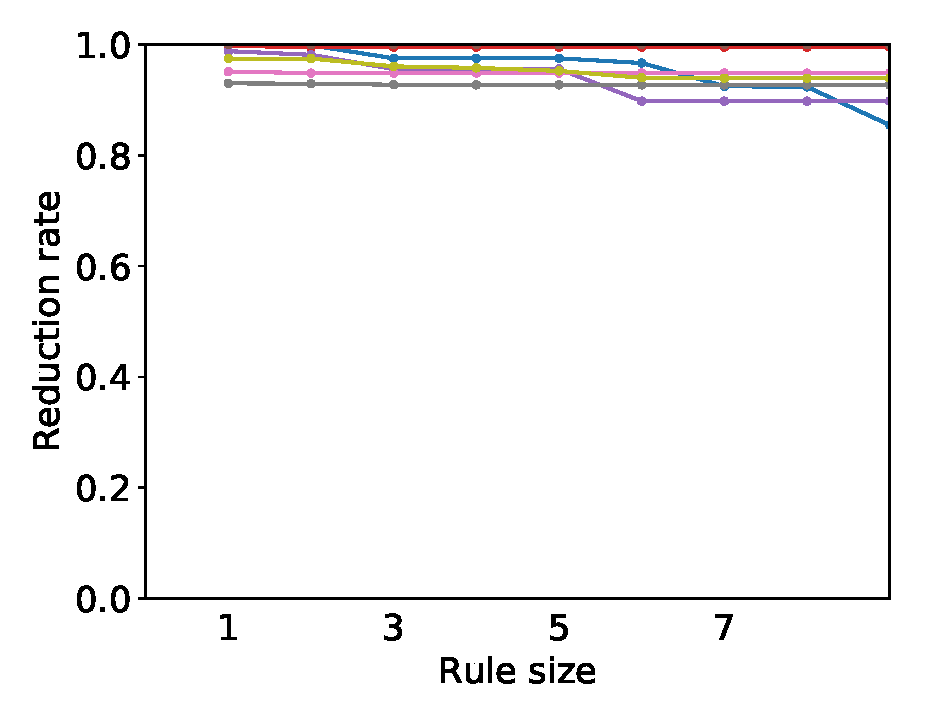
\includegraphics[scale=\subfigscale]{fig/chai/NELL-AR_rr}\label{fig:res-NELL-rr}}\\

%     \subfigure[EPSRC - Coverage]{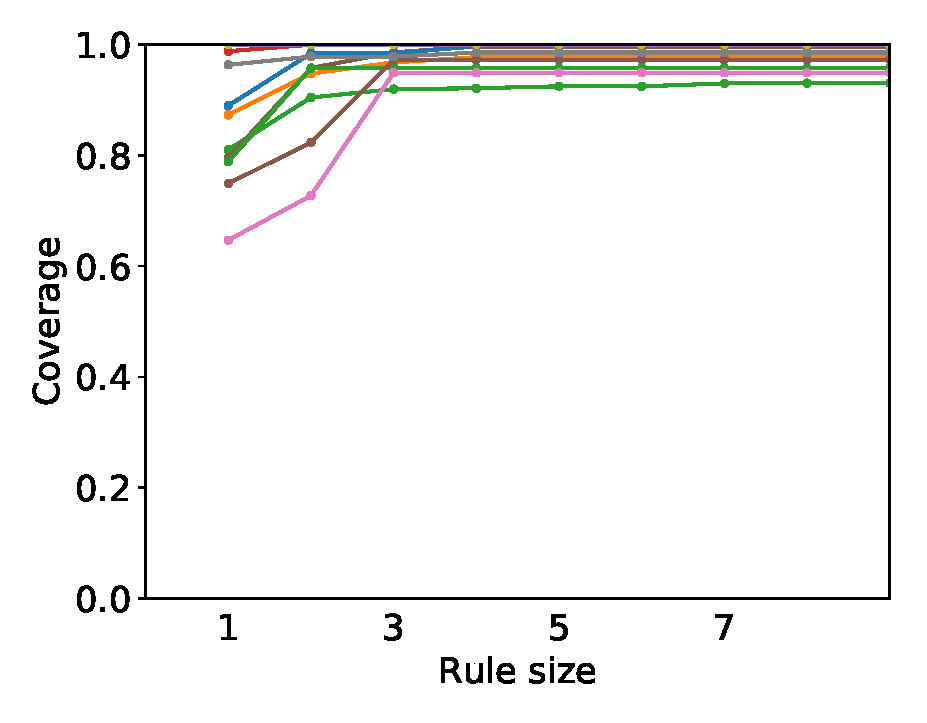
\includegraphics[scale=\subfigscale]{fig/chai/epsrc_recall}\label{fig:res-EPSRC-recall}}~
%     \subfigure[EPSRC - Reduction rate]{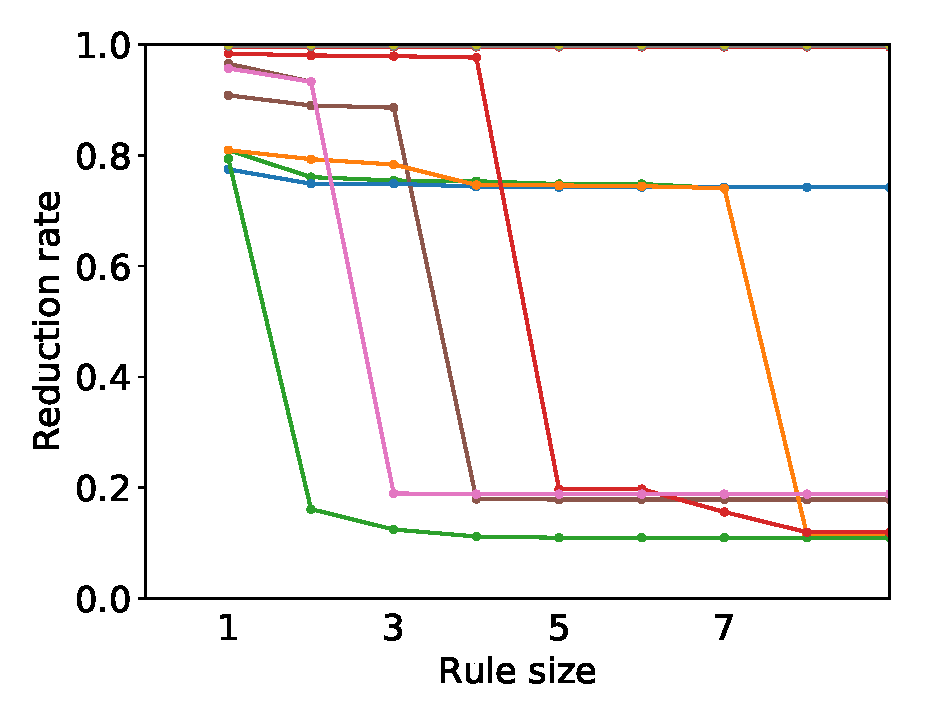
\includegraphics[scale=\subfigscale]{fig/chai/epsrc_rr}\label{fig:res-EPSRC-rr}}\\

%     \caption{Evolution of the coverage (left) and reduction rate (right) values}
%     \label{fig:chai-fitness-datasets}
% \end{figure*}

% \begin{figure}[htp]
%     \centering
%     \def\subfigscale{0.4}
%     \subfigure[FB13]{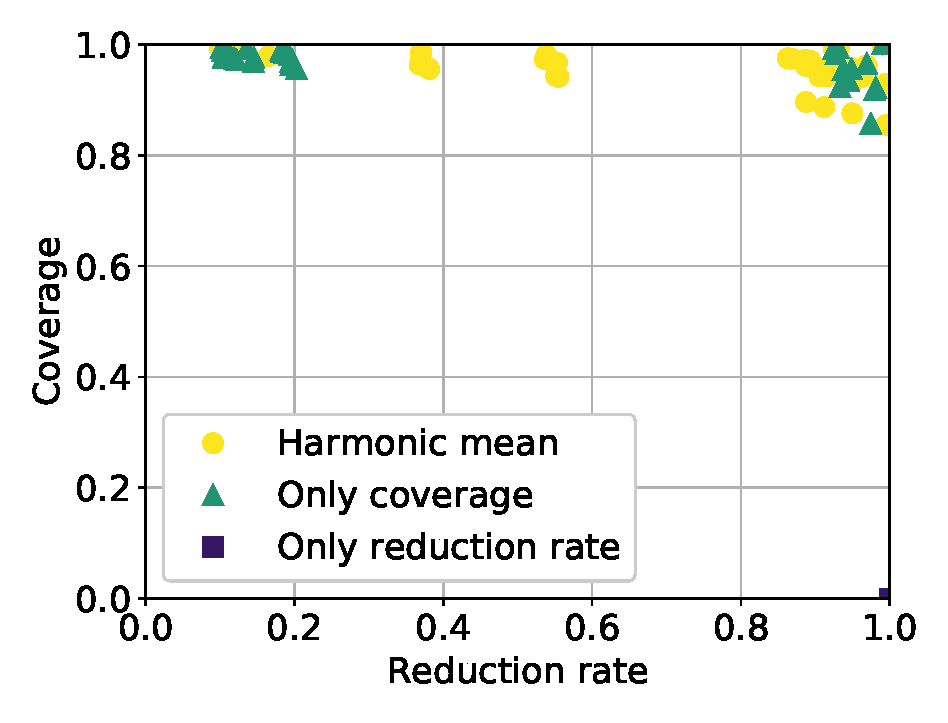
\includegraphics[scale=\subfigscale]{fig/chai/FB13_points}\label{fig:res-FB13-points}}~
%     \subfigure[WN18]{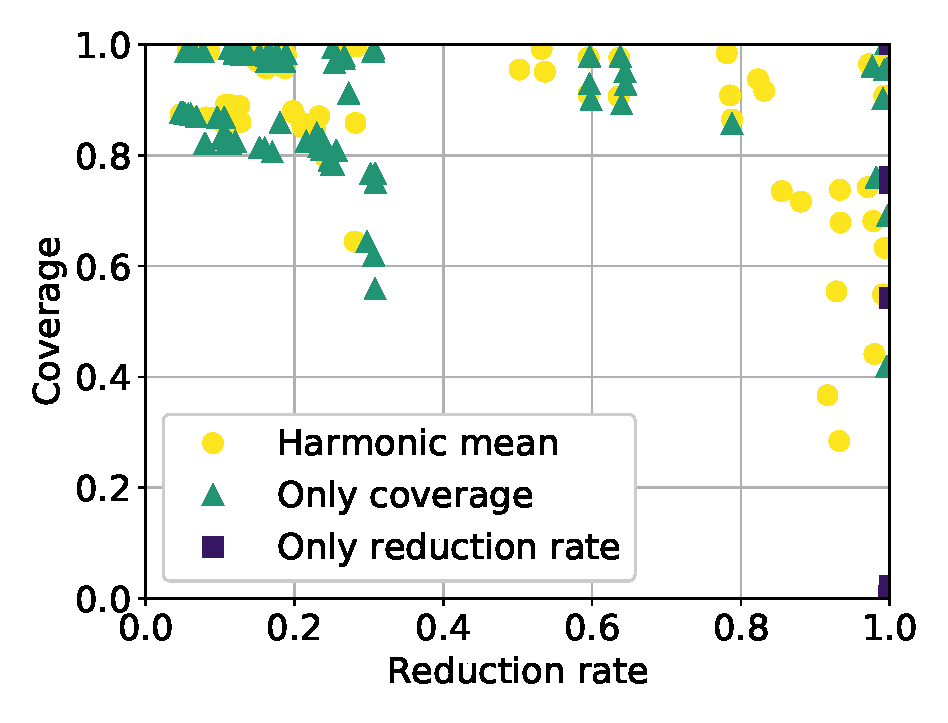
\includegraphics[scale=\subfigscale]{fig/chai/WN18-AR_points}\label{fig:res-WN18-points}}
%     \subfigure[NELL]{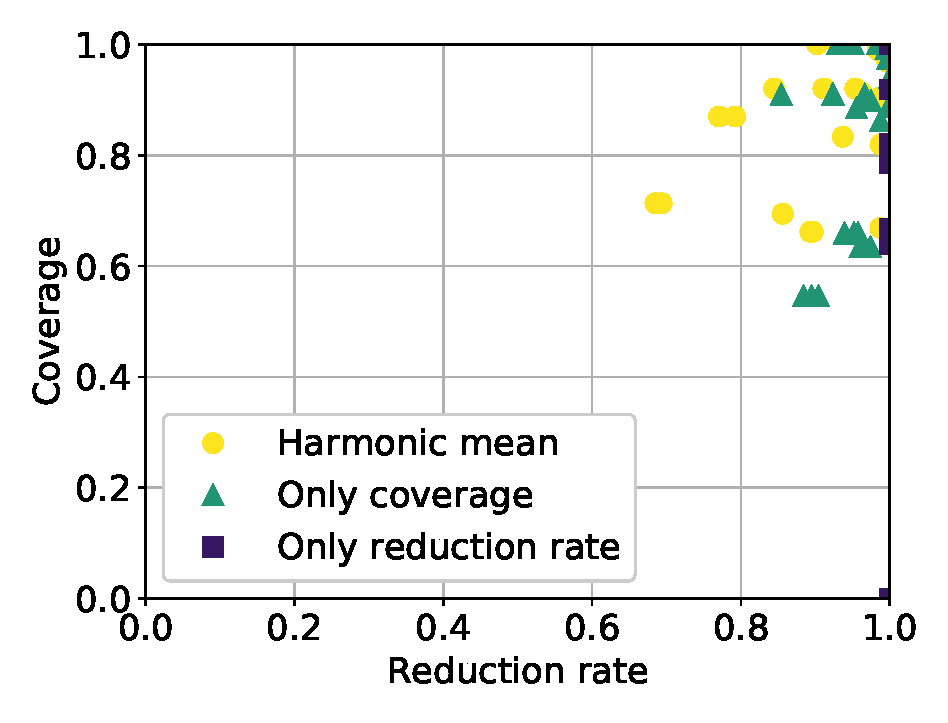
\includegraphics[scale=\subfigscale]{fig/chai/NELL-AR_points}\label{fig:res-NELL-points}}~
%     \subfigure[EPSRC]{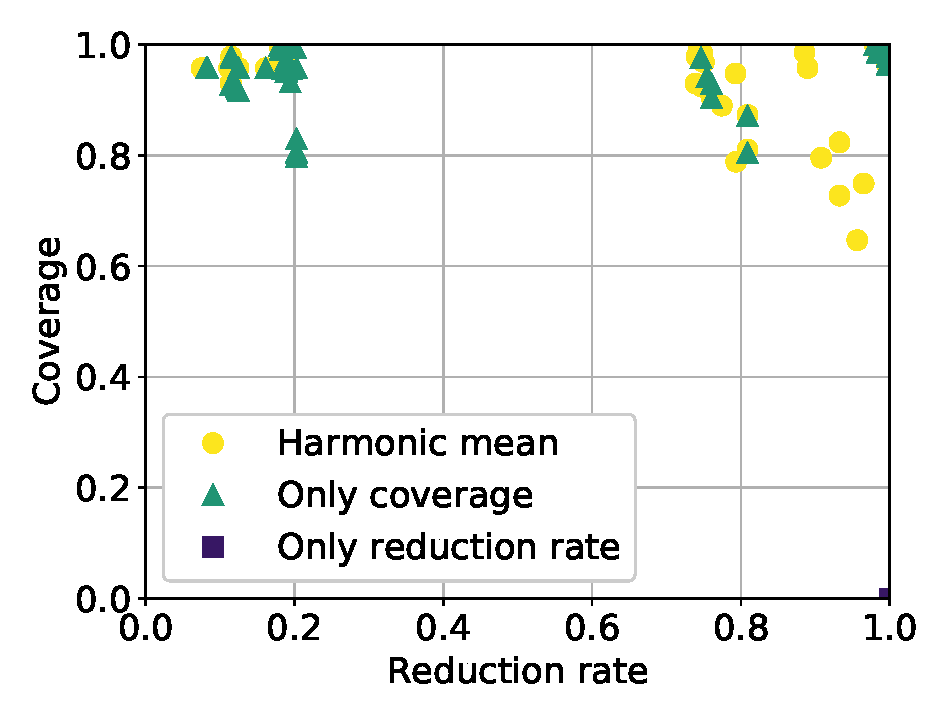
\includegraphics[scale=\subfigscale]{fig/chai/epsrc_points}\label{fig:res-EPSRC-points}}
%     \caption{Reduction rate (x) and coverage (y) for different fitness functions}
%     \label{fig:chai-points-datasets}
% \end{figure}

% \begin{table}[htp]
    \begin{center}
    \begin{tabular}{ M{1.5cm} | M{2.5cm} | M{2.5cm} | M{2.5cm} | M{2.5cm} } 
    \centering \textbf{KG} & \textbf{Avg. max. coverage (CHAI)} & \textbf{Avg. coverage (baseline)} & \textbf{Avg. max. RR (CHAI)} & \textbf{Avg. RR (baseline)} \\
    \hline
    FB13 & \textbf{0.92} (0.76-1.00) & \textbf{0.78} (0.58-0.99) & \textbf{0.91} (0.76-1.00) & \textbf{0.91} (0.76-1.00) \\ 
    \hline 
    WN18 & \textbf{0.94} (0.89-0.99) & \textbf{0.49} (0.26-0.72) & \textbf{0.97} (0.93-1.00) & \textbf{0.93} (0.85-1.00) \\
    \hline 
    NELL & \textbf{0.89} (0.78-1.00) & \textbf{0.53} (0.26-0.80) & \textbf{0.97} (0.95-1.00) & \textbf{0.99} (0.99-1.00) \\
    \hline 
    EPSRC & \textbf{0.99} (0.98-1.00) & \textbf{0.82} (0.68-0.97) & \textbf{0.95} (0.91-0.99) & \textbf{0.95} (0.92-0.99) \\
    \end{tabular}
    \end{center}
    \caption{Max. coverage and reduction rate values (avg and 95\% conf.)}
    \label{table:recall-rr-max}
\end{table}

% These results allow us to distinguish between two types of relations: those for which a high coverage value is obtained with a very short rule, and those for which the coverage starts at a lower value and increments as rules grow in size, as shown in Figure \ref{fig:chai-fitness-datasets}. We consider the former type of relations to be categorical, as they have a range of possible target entities that is relatively small: for example, the entities that are targets for the relation \textit{location} are unlikely to appear as the target for any other relation, and thus using the entities that are targets for \textit{location} as possible candidates for locations yields a very good result. On the other hand, relations that are non-categorical have a much wider range of possible candidates: in the case of the relation \textit{children}, an entity may produce a good candidate even if it does not appear as the target of \textit{children} (for example, they may appear in the relation \textit{sibling}).

% This conclusion is reinforced by the results shown in Figure \ref{fig:chai-points-datasets}, where there are groups of iterations in the top-right corner (the area of both high reduction rate and high coverage), which are obtained for categorical relations with a small subset of possible targets, while a different group of iterations show more scattered results in the top area, denoting that in order to achieve a high coverage, a bigger set of candidates must be used (non-categorical relations). Additionally, the results shown in this Figure lead us to the conclusion that using only reduction rate as the fitness function results in a very poor coverage, as the algorithm stops after having selected only one criterion that allows a very small number of candidates. On the contrary, using only coverage as the fitness function provides better results, but with a clear tendency towards prioritizing coverage at the expense of a lower reduction rate, while using the harmonic mean yields more balanced results.

% In the case of non-categorical relations, there exists a trade-off between coverage and reduction rate. This is to be expected, since rules are disjunctions of criteria and thus rules that comprise more criteria are more likely to filter out less candidates, increasing coverage but decreasing the reduction rate. In these cases, it is up to the user to decide whether they are interested in achieving a very high coverage with a lower reduction rate, or a higher reduction rate with a usually lower coverage. For this kind of relations, distance-based criteria are generally useful: for example, one's parents or spouse are usually found within a short distance in the KG. In categorical relations, however, one is able to obtain both a high reduction rate and a high coverage, because the entities that are suitable targets for said relations can easily be found by analyzing the domains and ranges of the relation in question or other relations.

% Regarding the reduction rate, it must be noted that it is computed with regard to the set of candidates that are selected by the $exists$ criterion, and not with respect to the Cartesian product of all possible candidates. This results in reduction rates that are in all cases lower than those that would be obtained in the latter case, though more evenly spread between 0 and 1. Given that high reduction rates are still achieved, we do not consider this to be a problem, but rather an adequate way of measuring how many candidates are selected with respect to an initial set of filtered candidates, with many unlikely candidates already filtered out.

% Finally, it is worth noting that CHAI consistently manages to achieve high coverage values for all Knowledge Graphs under study, as it can be seen in Figure \ref{fig:chai-fitness-datasets}. These values start to converge with rules composed of approximately five criteria, and thus we find that the criteria that are ranked higher by means of the proposed fitness function (Eq. \ref{eq:fitness-recall-rr}) are indeed successful in allowing promising candidates to pass the filter. When comparing CHAI to the baseline approach proposed by \citet{shi18}, CHAI achieves much higher values of coverage while still being able to obtain similar reduction rates, as shown in Table \ref{table:recall-rr-max}. The values for CHAI shown in said Table refer to the average maximum values that can be achieved, and thus our proposal is more versatile as it allows the user to prioritize a higher coverage by using longer rules, or a higher reduction rate by using shorter rules. CHAI works well for all kinds of relations due to the versatility of the criteria it uses, while the proposal by \citet{shi18} is not able to deal as effectively with non-categorical relations in terms of coverage, hindering its overall performance.


\section{Limitations}\label{sec:chai-limitations}
% While CHAI obtains satisfactory results, it is not without limitations. Perhaps the most important one would arise in the case of a KG with a very high number of total relations, because the amount of domain and range-based criteria would be equally high. In this case, the fitness function would have to be computed for every criterion in order to sort them by decreasing fitness value, resulting in a potentially high computational cost. Besides, CHAI may not work as well in very sparse KGs where all or most relations share the same entities in their domains and ranges, because the distance-based criterion would need a much higher threshold due to the sparsity of possible paths, and the domain and range-based ones would not prove useful.

\section{Summary}\label{sec:chai-summary}
In this chapter we have introduced CHAI, our proposal to filter candidate triples for Knowledge Graph completion. CHAI works by producing candidate filtering rules by combining a set of criteria in such a way that it optimizes a fitness function. Furthermore, CHAI produces a rule for every distinct relation in the KG, thus ensuring that the result of applying such rules is specifically tailored to the nature of every relation. Our experimental evaluation shows that CHAI is effective in practice, producing sets of candidate triples that are considerably smaller than other state-of-the-art approaches to this task, while still containing most of the candidates that could be considered promising.